\documentclass[11pt,letter, swedish, english
]{article}
\pdfoutput=1

\usepackage{../custom_as}
\usepackage[makeroom
]{cancel}
\graphicspath{{figures/}}

\swapcommands{\Delta}{\varDelta}
\swapcommands{\Omega}{\varOmega}

%%Drar in tabell och figurtexter
\usepackage[margin=10 pt]{caption}
%%För att lägga in 'att göra'-noteringar i texten
\usepackage{todonotes} %\todo{...}

%%För att själv bestämma marginalerna. 
\usepackage[
%            top    = 2.5cm,
%            bottom = 3cm,
%            left   = 3cm, right  = 3cm
]{geometry}

%%För att ändra hur rubrikerna ska formateras


\renewcommand{\thefootnote}{\fnsymbol{footnote}}

\newcommand{\Tc}{\ensuremath{T_{\text{c}}}}
\newcommand{\sign}{\ensuremath{\text{sign}}}

%\usepackage{tikz}

\begin{document}

%\tikzstyle{every picture}+=[remember picture]
%\tikzstyle{na} = [shape=rectangle,inner sep=0pt,text depth=0pt]



%%%%%%%%%%%%%%%%% vvv Inbyggd titelsida vvv %%%%%%%%%%%%%%%%%

\title{Statistical Physics 2 -- PHYS\,705 \\
Assignment 1}
\author{Andréas Sundström}
\date{\today}

\maketitle

%%%%%%%%%%%%%%%%% ^^^ Inbyggd titelsida ^^^ %%%%%%%%%%%%%%%%%

\section{Mean field magnetic susceptibility}
\renewcommand{\thesubsection}{\arabic{section} (\roman{subsection})}

In this problem, we will study the magnetic susceptibility, $\chi$, in
view of the MFT approach to the Ising model. We will look at the
asymptotic behaviour of $\chi$ for $T\to0^+$ and $T\to\Tc$.

We begin from the MF equation
\begin{equation}\label{eq:1_MFE}
M=\tanh(\frac{MJ + B}{T}),
\end{equation}
and the definition of susceptibility
\begin{equation}\label{eq:1_chi}
\chi:=\eval{\dv{M}{B}}_{B=0}.
\end{equation}

By applying \eqref{eq:1_chi} to \eqref{eq:1_MFE}, we get
\begin{equation}
\chi=\frac{1}{\cosh^2(MJ/T)}\, 
\qty(\frac{J}{T}\chi+\frac{1}{T}),
\end{equation}
or in other words
\begin{equation}\label{eq:1_chi_exact}
\chi=\frac{1}{T\cosh^2(M\Tc/T)-\Tc}.
\end{equation}
In the last step we also used the fact that $\Tc=J$ using the MFT approach.

\subsection{Zero temperature limit}
As $T\to0^+$, the leading order behaviour of the hyperbolic cosine is
\begin{equation}
\cosh^2\qty(\frac{M\Tc}{T})\sim \frac{1}{4}\exp(2\frac{\abs{M}\Tc}{T}).
\end{equation}
This exponential growth will dominate over the factor $T$ in
front and the constant $-\Tc$ in the denominator. And \eqref{eq:1_MFE}
also shows us that $M\to\pm1$ as $T\to0^+$. 

The asymptotic behaviour of \eqref{eq:1_chi_exact} will be 
\begin{equation}
\chi\sim \frac{4}{T}\exp(-2\frac{\Tc}{T})
\qcomma \text{as}\ T\to0.
\end{equation}
And to be clear, this asymptotic behaviour results in $\chi(T)\to0$ as
$T\to0$. 


\subsection{Critical temperature limit}
We begin with aproaching the limit from below, $T<\Tc$. We do still
evaluate the derivative for $\chi$ at $B=0$, so the MFT value for $M$
can be used:
\begin{equation}
M=\sqrt{3}\frac{T}{\Tc}\sqrt{-t}.
\end{equation}
Plugging this into the exact expression \eqref{eq:1_chi_exact} and
Taylor expanding the hyperbolic cosine gives
\begin{equation}
\begin{aligned}
\chi(T\to\Tc^-)\sim&\frac{1}{T\qty[1+3(T/\Tc)^2(\Tc-T)/\Tc]-\Tc}\\
=&\frac{1}{T-3(T/\Tc)^3(T-\Tc) -\Tc}\\
=&\frac{1}{T-\Tc}\times\frac{1}{1-3(T/\Tc)^3}\\
\sim&\frac{1}{2}\times\frac{1}{\Tc-T}=\frac{1}{2\Tc}|t|^{-1}.
\end{aligned}
\end{equation}
If we approach the limit from the other end, we know that $M=0$. So
\eqref{eq:1_chi_exact} is just
\begin{equation}
\chi(T\to\Tc^+)=\frac{1}{T-\Tc}=\frac{1}{\Tc} |t|^{-1}.
\end{equation}

To conclude this part of the problem we note that in both cases, we
can write
\begin{equation}
\chi=C_\pm |t|^{-\gamma},
\end{equation}
where $\gamma=1$ and $C_+/C_-=2$.



\section{Phase transitions in Landau theory}
\renewcommand{\thesubsection}{\arabic{section} (\alph{subsection})}
\renewcommand{\thesubsubsection}{\arabic{section} (\alph{subsection},\,\roman{subsubsection})}

Here, we will use the Landau free energy
\begin{equation}\label{eq:2_F(M)}
F=-bM+tM^2+uM^4+M^6,
\end{equation}
where $b=B/T$, $t=(T-\Tc)/\Tc$ and $u$ is some coefiicient with no
restrictions. 

\subsection{Generic forms of $F$}
There will be, depending on how precise you want to be, around four
different generic forms of $F$, and they occur at
\begin{enumerate}[label=\Roman*.]
\item $t\ge0$, $u\ge0$ \\
Here, it's obvious that all we can get is a single minimum at $M=0$.
\item $t<0$, $u$ any value; or $t=0$, $u<0$\\
For $t<0$, the initial behaviour around $M=0$ is to drop down, but at
large $|M|$ we still get $F\to+\infty$. So we must have two minima at
$M\neq0$, and a local maximum at $M=0$. The same is true for $t=0$ and
$u<0$. 
\item $0<t<u^2/4$, $u<0$\footnotemark{}\addtocounter{footnote}{-1}\\
Here, we initially get a growing $F$, near $M=0$, but the effects of a
negative enough $u$ will then come into play and force down $F(m)$ to
two minima at $M\neq0$ which are stronger than the one at $M=0$.
\item $t>u^2/4$, $u<0$\footnotemark{}\\
In this case, there might not even be two minima at $M\neq0$, but if
they excist they are weaker than the one at $M=0$.
\end{enumerate}
These four cases encompass all of the $u{-}T$ plane. The generic forms
of $F(M)$ can be seen in \figref{fig:2a}.

\footnotetext{The difference between these two cases will be
  further elaborated on in part (b) of this problem.}

\begin{figure}
\centering
% GNUPLOT: LaTeX picture with Postscript
\begingroup
  \makeatletter
  \providecommand\color[2][]{%
    \GenericError{(gnuplot) \space\space\space\@spaces}{%
      Package color not loaded in conjunction with
      terminal option `colourtext'%
    }{See the gnuplot documentation for explanation.%
    }{Either use 'blacktext' in gnuplot or load the package
      color.sty in LaTeX.}%
    \renewcommand\color[2][]{}%
  }%
  \providecommand\includegraphics[2][]{%
    \GenericError{(gnuplot) \space\space\space\@spaces}{%
      Package graphicx or graphics not loaded%
    }{See the gnuplot documentation for explanation.%
    }{The gnuplot epslatex terminal needs graphicx.sty or graphics.sty.}%
    \renewcommand\includegraphics[2][]{}%
  }%
  \providecommand\rotatebox[2]{#2}%
  \@ifundefined{ifGPcolor}{%
    \newif\ifGPcolor
    \GPcolortrue
  }{}%
  \@ifundefined{ifGPblacktext}{%
    \newif\ifGPblacktext
    \GPblacktexttrue
  }{}%
  % define a \g@addto@macro without @ in the name:
  \let\gplgaddtomacro\g@addto@macro
  % define empty templates for all commands taking text:
  \gdef\gplbacktext{}%
  \gdef\gplfronttext{}%
  \makeatother
  \ifGPblacktext
    % no textcolor at all
    \def\colorrgb#1{}%
    \def\colorgray#1{}%
  \else
    % gray or color?
    \ifGPcolor
      \def\colorrgb#1{\color[rgb]{#1}}%
      \def\colorgray#1{\color[gray]{#1}}%
      \expandafter\def\csname LTw\endcsname{\color{white}}%
      \expandafter\def\csname LTb\endcsname{\color{black}}%
      \expandafter\def\csname LTa\endcsname{\color{black}}%
      \expandafter\def\csname LT0\endcsname{\color[rgb]{1,0,0}}%
      \expandafter\def\csname LT1\endcsname{\color[rgb]{0,1,0}}%
      \expandafter\def\csname LT2\endcsname{\color[rgb]{0,0,1}}%
      \expandafter\def\csname LT3\endcsname{\color[rgb]{1,0,1}}%
      \expandafter\def\csname LT4\endcsname{\color[rgb]{0,1,1}}%
      \expandafter\def\csname LT5\endcsname{\color[rgb]{1,1,0}}%
      \expandafter\def\csname LT6\endcsname{\color[rgb]{0,0,0}}%
      \expandafter\def\csname LT7\endcsname{\color[rgb]{1,0.3,0}}%
      \expandafter\def\csname LT8\endcsname{\color[rgb]{0.5,0.5,0.5}}%
    \else
      % gray
      \def\colorrgb#1{\color{black}}%
      \def\colorgray#1{\color[gray]{#1}}%
      \expandafter\def\csname LTw\endcsname{\color{white}}%
      \expandafter\def\csname LTb\endcsname{\color{black}}%
      \expandafter\def\csname LTa\endcsname{\color{black}}%
      \expandafter\def\csname LT0\endcsname{\color{black}}%
      \expandafter\def\csname LT1\endcsname{\color{black}}%
      \expandafter\def\csname LT2\endcsname{\color{black}}%
      \expandafter\def\csname LT3\endcsname{\color{black}}%
      \expandafter\def\csname LT4\endcsname{\color{black}}%
      \expandafter\def\csname LT5\endcsname{\color{black}}%
      \expandafter\def\csname LT6\endcsname{\color{black}}%
      \expandafter\def\csname LT7\endcsname{\color{black}}%
      \expandafter\def\csname LT8\endcsname{\color{black}}%
    \fi
  \fi
  \setlength{\unitlength}{0.0500bp}%
  \begin{picture}(9070.00,8502.00)%
    \gplgaddtomacro\gplbacktext{%
      \csname LTb\endcsname%
      \put(192,6220){\rotatebox{-270}{\makebox(0,0){\strut{}$F(M, t, u)$}}}%
      \put(2267,4419){\makebox(0,0){\strut{}$M$}}%
      \put(2267,8141){\makebox(0,0){\strut{}I. $t\ge0$, $u\ge0$}}%
    }%
    \gplgaddtomacro\gplfronttext{%
    }%
    \gplgaddtomacro\gplbacktext{%
      \csname LTb\endcsname%
      \put(4727,6220){\rotatebox{-270}{\makebox(0,0){\strut{}$F(M, t, u)$}}}%
      \put(6802,4419){\makebox(0,0){\strut{}$M$}}%
      \put(6802,8141){\makebox(0,0){\strut{}II. $t<0$, $u$ any value; or $t=0$, $u<0$}}%
    }%
    \gplgaddtomacro\gplfronttext{%
    }%
    \gplgaddtomacro\gplbacktext{%
      \csname LTb\endcsname%
      \put(192,1969){\rotatebox{-270}{\makebox(0,0){\strut{}$F(M, t, u)$}}}%
      \put(2267,168){\makebox(0,0){\strut{}$M$}}%
      \put(2267,3891){\makebox(0,0){\strut{}III. $0<t<u^2/4$, $u<0$}}%
    }%
    \gplgaddtomacro\gplfronttext{%
    }%
    \gplgaddtomacro\gplbacktext{%
      \csname LTb\endcsname%
      \put(4727,1969){\rotatebox{-270}{\makebox(0,0){\strut{}$F(M, t, u)$}}}%
      \put(6802,168){\makebox(0,0){\strut{}$M$}}%
      \put(6802,3891){\makebox(0,0){\strut{}IV. $t>u^2/4$, $u<0$}}%
    }%
    \gplgaddtomacro\gplfronttext{%
      \csname LTb\endcsname%
      \put(7854,891){\makebox(0,0)[r]{\strut{}$t>u^2/4$, but not by much}}%
      \csname LTb\endcsname%
      \put(7854,651){\makebox(0,0)[r]{\strut{}$t\gg u^2/4$}}%
    }%
    \gplbacktext
    \put(0,0){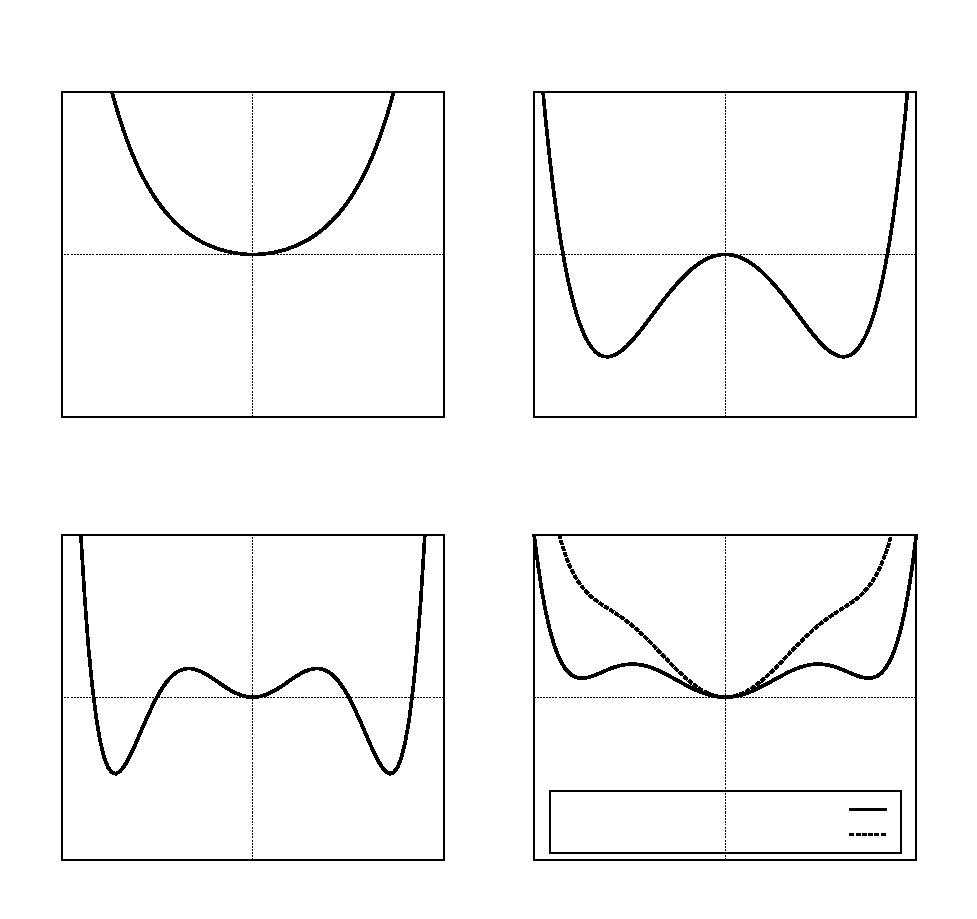
\includegraphics{generic_forms}}%
    \gplfronttext
  \end{picture}%
\endgroup

\caption{The four (or five) different generic forms of $F(M)$, as
  given by \eqref{eq:2_F(M)}. }
\label{fig:2a}
\end{figure}

\subsection{First order transition, when $u<0$}
As illustrated in the difference between case III and IV, we see that
when $u<0$ it is indeed possible to get a scenario when the global
minimum of $F(M)$ jumps from $M=0$ to $\pm M_0\neq0$. The transition
occurs when the equation 
\begin{equation}
tM^2+uM^4+M^6=M^2(t+uM^2+M^4)=0
\end{equation}
goes from only one real solution to three/five. This is because we
know that the minimum at $M=0$ gives $F(M=0)=0$. So if we were to get
more solutions to this equation, that would mean that $F$ can assume
negative values. Ergo, there are some other minima which are stronger
than the one at $M=0$. 

We are therefore looking for when
\begin{equation}
t+uM^2+M^4=0
\end{equation}
starts having real solutions. These solutions are
\begin{equation}
M^2=\frac{-u\pm\sqrt{u^2-4t}}{2},
\end{equation}
and we see that this occurs only if $t\le u^2/4$. We are now in case
III, where the \emph{global} minima is away from $M=0$. But $M=0$ is
still however a \emph{local} minimum; this means that there is a
chance that the system will remain in $M=0$ all the way until $t=0$,
when we enter case II. In case II, $M=0$ is instead a local maximum so the
system will quickly find its way to one of the two minima with
non-zero $M$. 

% Note also that the temperature at which this sudden jump in
% magetization happens is at $t=u^2/4>0$. That is the phase
% transition occurs at a temerature above $\Tc$.


\subsection{The tri-critical point}

\subsubsection{Phase transitions}
From the analysis in the previous part of the problem, we know that
the line of the first order transition is at $t=u^2/4$. This is
however only valid for $u<0$, so the first order transition line ends
at $(t, u)=(0, 0)$; that is the tri-critical point.

The second order phase transition is on the $t=0$ line with
$u\ge0$. All of this is ilustrated in \figref{fig:2_phase}.

\begin{figure}\centering
\input{figures/phase_diagram.pdf_t}
\caption{A phase diagram showing the reagions where the different
  cases, from the previous figure, are located. Case I and IV are 
  uncondensed, whereas case II and III are condensed phases. There
  might be some hysterisis involved in case III. }
\label{fig:2_phase}
\end{figure}

\subsubsection{Critical exponents}
Here we're going to find the critical exponents as we approach the
tri-critical point along the $u=0$ line. 

Let's begin by $\beta$. For this we need to know
$M(t,B=0)\propto(-t)^\beta$. We just use \eqref{eq:2_F(M)} and
differentiate both sides, remembering that $u=b=0$:
\begin{equation}\label{eq:2ii_M}
2tM+6M^5=0\quad\Longrightarrow\quad
M=\qty(-\frac{1}{3}t)^{1/4}.
\end{equation}
So $\beta=1/4$.

Next is $\gamma$: $\chi=C_\pm|t|^{-\gamma}$. To get $\chi$ we need to
keep the term involving $b$ when we calculate $M$:
\begin{equation}\label{eq:2ii_gamma}
-b+2tM+6M^5=0.
\end{equation}
For $t>0$, we can assume that $M\ll1$ which means that the $M^5$ term
can be disregarded ($M^5\lll1$). This gives us $M=b/(2t)$ or
\begin{equation}
\chi(T\to\Tc^+)=\frac{1}{2t}.
\end{equation}
For $t<0$, we need a bit more work.
Assuming $b\ll t$, we can use perturbation theory and write
$M(b)=M_0+bM_1+\ldots$. By substituing this into \eqref{eq:2ii_gamma},
we get
\begin{equation}
\begin{aligned}
0=&-b+2t(M_0+bM_1)+6(M_0+bM_1)^5+\order{b^2}\\
=& \qty(M_0+6M_0^5)+b\qty(-1+2tM_1+30M_0^4M_1) +\order{b^2}.
\end{aligned}
\end{equation}
The unperturbed solution $M_0$ is just what we got in
\eqref{eq:2ii_M}, and since the above equation should hold for any
$b$ we have
\begin{equation}
\qty(-1+2tM_1+30M_0^4M_1)=0 \quad\Longrightarrow\quad
M_1=\frac{1}{2t+30M_0^4}=\frac{1}{8|t|}.
\end{equation}
So in this case we got $\gamma=1$, and $C_+/C_-=4$.

Next we can take $\alpha$:
$C_V=-T\dv*[2]{F}{T}=A_\pm|t|^{-\alpha}$. For $t>0$, we have $\dv{M}{T}=0$
meaning that $\dv[2]{F}{T}=0$. For $t<0$ however, we get $M$ as in
\eqref{eq:2ii_M} which results in
\begin{equation}
F(t<0, u=0, b=0)=t(-\frac{1}{3}t)^{1/2}+(-\frac{1}{3}t)^{3/2}
=-\frac{2}{3\sqrt{3}}(-t)^{3/2}.
\end{equation}
This, in turn, gives
\begin{equation}
C_V=-T\dv[2]{F}{(-t)}\qty(\dv{(-t)}{T})^2=\ldots
=\frac{T}{2\sqrt{3}\Tc}|t|^{-1/2}.
\end{equation}
So here we got $\alpha=1/2$, $A_-=1/(2\sqrt{3})$ and $A_+=0$.

And lastly we have $\delta$: $M(b,t=0)\propto b^{1/\delta}$. This time
we can again use \eqref{eq:2ii_gamma}, but with $t=0$, which gives
\begin{equation}
M=\qty(\frac{1}{6}b)^{1/5},
\end{equation}
or in other words $\delta=5$.



\section{1D Ising model}
We begin with the (1D) Ising model
\begin{equation}\label{eq:3_H}
H=-J\sum_{i=1}^{N}\sigma_{i}\sigma_{i+1}-B\sum_{i=1}^N\sigma_i,
\end{equation}
where $\sigma_i=\pm1$. We have $N$ lattice sites, and periodic pondary
conditions which means that the coupling
$\sigma_N\sigma_{N+1}=\sigma_N\sigma_1$. 

From this we want to write down the free
energy when $B=0$ and when $B\neq0$. In both cases we will want to
knwo the partition function
\begin{equation}\label{eq:3_Z}
Z=\Tr{\ee^{\beta H}}
=\sum_{\sigma_1=\pm1}\sum_{\sigma_2=\pm1}\cdots\sum_{\sigma_N=\pm1}\ee^{-\beta H}.
\end{equation}

\subsection{No magnetic field}
We want a way to represent $\ee^{-\beta H}$, and since $H$ itself
consits of a sum we have
\begin{equation}
\ee^{-\beta H}=
\ee^{\beta J\sigma_1\sigma_2}\ee^{\beta J\sigma_2\sigma_3}
\cdots\ee^{\beta J\sigma_{N-1}\sigma_N}.
\end{equation}
To represent this product we can create a \emph{transfer matrix}
$T$ with elements
\begin{equation}\label{eq:3_T_sigma}
\mel{\sigma_i}{T}{\sigma_j}=\ee^{\beta J\sigma_i\sigma_j},
\end{equation}
which results in
\begin{equation}\label{eq:3_e^H_mel}
\ee^{-\beta H}=\mel{\sigma_1}{T}{\sigma_2}\mel{\sigma_2}{T}{\sigma_3}
\cdots\mel{\sigma_{N-1}}{T}{\sigma_N}\mel{\sigma_{N}}{T}{\sigma_1}.
\end{equation}

The really elegant thing about this is that when we put
\eqref{eq:3_e^H_mel} into all of the summs we get lots of
\emph{identities} --- that is 
\begin{equation}
\sum_{\sigma_2}\bra{\sigma_1}{T}
\overbrace{\ket{\sigma_2}\bra{\sigma_2}}^{=1}
{T}\ket{\sigma_3}
=\mel{\sigma_1}{T^2}{\sigma_3}.
\end{equation}
So the partition function becomes
\begin{equation}
\begin{aligned}
Z=&\sum_{\sigma_1}\sum_{\sigma_2}\cdots\sum_{\sigma_N}
\mel{\sigma_1}{T}{\sigma_2}\mel{\sigma_2}{T}{\sigma_3}
\cdots\mel{\sigma_{N-1}}{T}{\sigma_N}\mel{\sigma_{N}}{T}{\sigma_1}\\
=&\sum_{\sigma_1}\mel{\sigma_1}{T^N}{\sigma_1}
=\Tr{T^N}=\lambda_1^N+\lambda_2^N,
\end{aligned}
\end{equation}
where $\lambda_n$ are the eigenvalues of $T$ --- there are only two
eigenvalues because $\sigma_i$ only has two values. 

To calculate the eigenvalues of $T$, we use \eqref{eq:3_T_sigma} to
see that
\begin{equation}
T=\begin{pmatrix}
\ee^{\beta J} &\ee^{-\beta J}\\
\ee^{-\beta J} & \ee^{\beta J}
\end{pmatrix}
\end{equation}
in the $\sigma$ representation/basis. Now it's just a matter of
turning the crank to get the eigenvalues:
\begin{equation}
\begin{aligned}
&0=\det(T-\lambda I)=\qty(\ee^{\beta J}-\lambda)^2-\ee^{-2\beta J}\\
\Longrightarrow\quad&
\lambda=\ee^{\beta J}\pm\ee^{-\beta J}
=2\cosh(\beta J)\qcomma 2\sinh(\beta J). 
\end{aligned}
\end{equation}

We now have the free energy
\begin{equation}
F=-T\ln(Z)=-T\ln(\lambda_1^N+\lambda_2^N)
=-T\ln(2^N\qty[\cosh^N(\beta J) + \sinh^N(\beta J)]).
\end{equation}
If we want to, we can get an asymptotic behaviour in the thermodynamic
limit of $N\to\infty$, then the $\cosh^N(\beta J)\gg\sinh^N(\beta
J)$, and
\begin{equation}
F\sim-NT\ln(2\cosh(\beta J))
\qcomma \text{as }\ N\to\infty.
\end{equation}


\subsection{With magnetic field}
If we now have $B\neq0$, we need to add the magnetic field terms into
the reasoning. We want to use the transfer matrix method again, to do
that we rewrite the magnetic field coupling term in \eqref{eq:3_H} so
as to include both $\sigma_i$ and $\sigma_{i+1}$:
\begin{equation}
B\sum_{i=1}^N\sigma_i=\frac{1}{2}B\sum_{i=1}^N(\sigma_i+\sigma_{i+1}),
\end{equation}
again with $\sigma_{N+1}=\sigma_1$. 

Now we can write the new transfer matrix as
\begin{equation}
\mel{\sigma_i}{T}{\sigma_j}
=\exp[\beta J\sigma_i\sigma_j+\frac{\beta B}{2}(\sigma_i+\sigma_{i+1})].
\end{equation}
From here, we can once again write $\ee^{-\beta H}$ as in
\eqref{eq:3_e^H_mel}, and the same reasoning applies up to that we
need to calculate the new eigenvalues. Written out the transfermatrix
looks like
\begin{equation}
T=\begin{pmatrix}
\ee^{\beta (J+B)} &\ee^{-\beta J}\\
\ee^{-\beta J} & \ee^{\beta (J-B)},
\end{pmatrix}
\end{equation}
and has the eigenvalues (omitting the middle steps)
\begin{equation}\label{eq:3_lambda_pm}
\lambda_\pm=\ee^{\beta J}
\qty[\cosh(\beta B)\pm\sqrt{\sinh^2(\beta B)+\ee^{-4\beta J}}].
\end{equation}
Note that these eigenvalues generalize, by setting $B=0$, to the ones
in the previous part of this problem. 

The free energy is
\begin{equation}
F=-T\ln(\lambda_+^N+\lambda_-^N)
\end{equation}
with $\lambda_\pm$ as in \eqref{eq:3_lambda_pm}. The asymptotic
behaviour, as $N\to\infty$, is (because $\lambda_+>\lambda_-$)
\begin{equation}
F\sim-TN\ln(\lambda_+)
=-JN -TN\ln(\cosh(\beta B)+\sqrt{\sinh^2(\beta B)+\ee^{-4\beta J}}).
\end{equation}

\subsubsection*{Magetization in this model}
The maroscopic magnetization per spin is
\begin{equation}
\begin{aligned}
M=&-\frac{1}{N}\pdv{F}{B}\\
=&T\frac{\beta\sinh(\beta B)
+\beta\sinh(\beta B)\cosh(\beta B)
\qty[\sinh^2(\beta B)+\ee^{-4\beta J}]^{-1/2}}
{\cosh(\beta B)+\sqrt{\sinh^2(\beta B)+\ee^{-4\beta J}}}\\
=&\frac{\sinh(\beta B)
+\sinh(\beta B)\cosh(\beta B)
\qty[\sinh^2(\beta B)+\ee^{-4\beta J}]^{-1/2}}
{\cosh(\beta B)+\sqrt{\sinh^2(\beta B)+\ee^{-4\beta J}}}.
\end{aligned}
\end{equation}

We therefore see that as $B\to0$ ($\beta$ finite), $\sinh(\beta
B)\to0$ and $\cosh(\beta B)\to1$; so $M\to0$ as $B\to0$ with a finite 
$\beta$. Whereas if we let $\beta\to\infty$ ($B\neq0$), we
get\footnotemark{} 
\begin{equation}
\begin{aligned}
M\sim&\frac{\sinh(\beta B)
+\sinh(\beta B)\cosh(\beta B)
\qty|\sinh(\beta B)|^{-1}}
{\cosh(\beta B)+|\sinh(\beta B)|}\\
=&\frac{\sinh(\beta B)+\sign(B)\cosh(\beta B)}
{\cosh(\beta B)+|\sinh(\beta B)|}\\
=&\sign(B)\frac{|\sinh(\beta B)|+\cosh(\beta B)}
{\cosh(\beta B)+|\sinh(\beta B)|}
=\sign(B).
\end{aligned}
\end{equation}
To conclude we have
\begin{equation}
M=\begin{cases}
0\quad&\text{if }\ T>0,\\
\pm1\quad&\text{if }\ T=0.
\end{cases}
\end{equation}
The $\pm$ is an artifact from when we still had some magnetic field,
but $\pm$ is still relevant in the end case since the spontaneously
broken symmetry equally well could have gone to $+1$ as to $-1$. 

\footnotetext{This is a bit abusive notation saying that $M$ is
  asymptotically 1 as $\beta\to\infty$, but this is physics and not
  math\ldots }


\section{Ising model generalization}
The simple Ising model only has a symmetry between positiv and
negative $\varphi$, therefor the Landau free enregy $F$ is expressed in
terms of $\varphi^2$. If we however consider a model with rotational
symmery in $n$ dimansions, we should still express $F$ in terms of
something invariant under rotations. The simplest such object is
$\varphi_i\varphi_i=\vb*{\varphi}\vdot\vb*{\varphi}$. And the Landau
free energy, in its simplest form, can be written as
\begin{equation}\label{eq:4_start}
F(\varphi_i)=-\vb*{b}\vdot\vb*{\varphi}+t\vb*{\varphi}\vdot\vb*{\varphi}
+(\vb*{\varphi}\vdot\vb*{\varphi})^2.
\end{equation}
The units are rescaled so that the coefficient in front of the
last term is $1$. 

In the absence of a magnetic field, there is no perfered
direction. And yet, the system will fall into a $\vb*\varphi$ pointing
in some direction --- spontaneous symmetry-breaking. Apart from the 1D
case, the direction of $\vb*\varphi$ can however change continuously. The only
restriction on $\vb*\varphi$ is that its magnitue is some specific
value, other than that $\vb*\varphi$ is free to rotate in any
direction. That is, the system keeps its symmetry; so the symmetry
isn't really broken here ($d\ge2$).

Since the system keeps its rotational symmetry in the absence of a
magnetic field, regardless of temperature, $\ev{\varphi_i}=0$. In the
case of $T<\Tc$, our analysis tells us that $|\vb*\varphi|=0$, so then
it's obvious that $\ev{\varphi_i}=0$. In the case of $T<\Tc$ however,
it's the rotational symmetry that will assure that $\varphi_i$ over
time will average out to 0. 

% As before, we see that (in the absence of $\vb*{b}$) the behaviour of
% $F$ is very similar to the 1D version. For instance, at $t>0$ the
% minimum of $F$ will occur at $\vb*{\varphi}\vdot\vb*{\varphi}=0$
% meaning that $\ev{\varphi_i}=0$. Where as when $t<0$, we would get
% some non-zero minimum where $|\vb*\varphi|=(-t/2)^{1/2}>0$ and
% \todo{Or should it be 0.}$\ev{\varphi_i}\neq0$ at least for some $i$'s. 




\subsubsection*{Critical exponents}
The critical exponents will be the same as for regular, 1D, Landau
theory since \eqref{eq:4_start} generalize to the 1D case and the
dimensionality of $\vb*\varphi$ won't affect the critical exponents. 
So let's just do the calculations in 1D\footnotemark{}.
\footnotetext{Another way of justifying this is to say that when the
  symmetry is broken, $\vb*\varphi = \varphi\vu*\lambda$ and use
  $\varphi=|\vb*\varphi|$ as the parameter in the following
  calculations. }

\begin{itemize}
\item[$\beta$: ] Minimizing $F(\varphi, b=0)=t\varphi^2+\varphi^4$,
gives $2t\varphi+4\varphi^3=0$ or $\varphi\propto(-t)^{\beta}$ where $\beta=1/2$.
\item[$\gamma$: ] Now we minimize $F(\varphi,
b)=-b\varphi+t\varphi^2+\varphi^4$: $-b+2t\varphi+4\varphi^3$. And if
we do it for $t>0$, we can disregard the cubic term to get
$\varphi\propto b/t$, which gives $\chi\propto[t]^{-\gamma}$ where
$\gamma=1$.
\item[$\alpha$: ] Here we calculate $C_V=-T\dv[2]{F}{T}$, with
$\varphi\propto(-t)^{1/2}$. This gives
$C_V\propto\dv[2]{t}t^2=\text{const.}$ or in other words
$C_V\propto|t|^{-\alpha}$ where $\alpha=0$.
\item[$\delta$: ] Here we want to minimize $F(t=0,
b)=-b\varphi+\varphi^4$, which gives $-b+4\varphi^3=0$ or
$\varphi\propto b^{1/\delta}$ where $\delta=3$.
\end{itemize}






\end{document}




%  LocalWords:  MFT MF
